%\documentclass[hyperref={pdfpagelabels=false},slidetop,9pt]{beamer}
\documentclass[slidetop,8pt]{beamer}
\usepackage[T1]{fontenc}
\usepackage[utf8]{inputenc}
\newcommand{\nom}{Porte conteneur}
\newcommand{\sequence}{03}
\newcommand{\num}{04}
\newcommand{\type}{TD}
\newcommand{\descrip}{Résolution d'un problème en utilisant des méthodes algorithmiques}
\newcommand{\competences}{Alt-C3: Concevoir un algorithme répondant à un problème précisément posé}
\usepackage{etex}
\usepackage{tikz}
\usepackage[european]{circuitikz}
\usepackage{pgf}
\usepackage[all]{xy}
\usepackage{pgfpages}
\usepackage{graphbox}
\usepackage{pdfpages}
\usepackage[adobe-utopia]{mathdesign}
\usepackage{ifthen}
\usepackage{cancel}
\usepackage{framed}
\usepackage{subfig}
\usepackage{tabularx}
\usepackage{setspace}
\usepackage{soul}
\usepackage{schemabloc}
\usepackage{eqnarray}
\usepackage[dot, phantomtext]{dashundergaps}
\usepackage{media9}
\usepackage{multimedia}

\author{Renaud Costadoat}
\institute{Lycée Dorian}

\usepackage{multido}
\usepackage{multirow}
\usepackage{multicol} % Portions de texte en colonnes
\usepackage{flafter}%floatants après la référence

\usepackage{color}
\usepackage{xcolor}
\usepackage{colortbl}

\usepackage[gen]{eurosym}
\usepackage{tikz}
%\usepackage{pstricks,pst-node,pst-tree,pst-solides3d}
\usepackage{lmodern}
\usepackage[francais]{babel}
\usepackage{pslatex}
\usetheme{renaud}
\usepackage{times}
\usepackage{amsmath}
\usepackage{verbatim}
\usepackage{moreverb}
%\usetikzlibrary{arrows,shapes}
\usepackage{graphicx}
\usepackage{psfrag}
\usepackage{wrapfig}
\usepackage{etoolbox}

\definecolor{gris25}{gray}{0.75}
\definecolor{bleu}{RGB}{18,33,98}
\definecolor{bleuf}{RGB}{42,94,171}
\definecolor{bleuc}{RGB}{231,239,247}
\definecolor{rougef}{RGB}{185,18,27}
\definecolor{rougec}{RGB}{255,188,204}%255,230,231
\definecolor{vertf}{RGB}{103,126,82}
\definecolor{vertc}{RGB}{220,255,191}

\setlength\parindent{24pt}
\parskip 7.2pt
\parindent 8pt

\newenvironment{rem}[1][\hsize]%
{%
    \def\FrameCommand
   {%
\rotatebox{90}{\textit{\textsf{Remarque}}} 
       {\color{bleuf}\vrule width 3pt}%
       \hspace{0pt}%must no space.
       \fboxsep=\FrameSep\colorbox{bleuc}%
  }%
    \MakeFramed{\hsize#1\advance\hsize-\width\FrameRestore}%
}%
{\endMakeFramed}%


\newenvironment{savoir}[1][\hsize]%
{%
    \def\FrameCommand
    {%
\rotatebox{90}{\textit{\textsf{Savoir}}} 
        {\color{bleuf}\vrule width 3pt}%
        \hspace{0pt}%must no space.
        \fboxsep=\FrameSep\colorbox{bleuc}%
    }%
    \MakeFramed{\hsize#1\advance\hsize-\width\FrameRestore}%
}%
{\endMakeFramed}%

\newenvironment{prob}[1][\hsize]%
{%
    \def\FrameCommand%
    {%
\rotatebox{90}{\textit{\textsf{Problématique}}} 
        {\color{rougef}\vrule width 3pt}%
        \hspace{0pt}%must no space.
        \fboxsep=\FrameSep\colorbox{rougec}%
    }%
    \MakeFramed{\hsize#1\advance\hsize-\width\FrameRestore}%
}%
{\endMakeFramed}%

\newenvironment{obj}[1][\hsize]%
{%
    \def\FrameCommand%
    {%
\rotatebox{90}{\textit{\textsf{Objectif}}} 
        {\color{vertf}\vrule width 3pt}%
        \hspace{0pt}%must no space.
        \fboxsep=\FrameSep\colorbox{vertc}%
    }%
    \MakeFramed{\hsize#1\advance\hsize-\width\FrameRestore}%
}%
{\endMakeFramed}%

\newenvironment{defi}[1][\hsize]%
{%
    \def\FrameCommand%
    {%
\rotatebox{90}{\textit{\textsf{Definition}}} 
        {\color{bleuf}\vrule width 3pt}%
        \hspace{0pt}%must no space.
        \fboxsep=\FrameSep\colorbox{rougec}%
    }%
    \MakeFramed{\hsize#1\advance\hsize-\width\FrameRestore}%
}%
{\endMakeFramed}%


\newenvironment{hypo}[1][\hsize]%
{%
    \def\FrameCommand%
    {%
\rotatebox{90}{\textit{\textsf{Hypothèse\\}}} 
        {\color{bleuf}\vrule width 3pt}%
        \hspace{0pt}%must no space.
        \fboxsep=\FrameSep\colorbox{bleuc}%
    }%
    \MakeFramed{\hsize#1\advance\hsize-\width\FrameRestore}%
}%
{\endMakeFramed}%


\newenvironment{prop}[1][\hsize]%
{%
    \def\FrameCommand%
    {%
\rotatebox{90}{\textit{\textsf{Propriété}}} 
        {\color{bleuf}\vrule width 3pt}%
        \hspace{0pt}%must no space.
        \fboxsep=\FrameSep\colorbox{bleuc}%
    }%
    \MakeFramed{\hsize#1\advance\hsize-\width\FrameRestore}%
}%
{\endMakeFramed}%

\newenvironment{props}[1][\hsize]%
{%
    \def\FrameCommand%
    {%
\rotatebox{90}{\textit{\textsf{Propriétés}}} 
        {\color{bleuf}\vrule width 3pt}%
        \hspace{0pt}%must no space.
        \fboxsep=\FrameSep\colorbox{bleuc}%
    }%
    \MakeFramed{\hsize#1\advance\hsize-\width\FrameRestore}%
}%
{\endMakeFramed}%

\newenvironment{exemple}[1][\hsize]%
{%
    \def\FrameCommand%
    {%
\rotatebox{90}{\textit{\textsf{Exemple}}} 
        {\color{vertf}\vrule width 3pt}%
        \hspace{0pt}%must no space.
        \fboxsep=\FrameSep\colorbox{vertc}%
    }%
    \MakeFramed{\hsize#1\advance\hsize-\width\FrameRestore}%
}%
{\endMakeFramed}%

\newenvironment{resultat}[1][\hsize]%
{%
    \def\FrameCommand%
    {%
\rotatebox{90}{\textit{\textsf{Resultat}}} 
        {\color{rougef}\vrule width 3pt}%
%        {\color{bleuf}\vrule width 3pt}%
        \hspace{0pt}%must no space.
        \fboxsep=\FrameSep\colorbox{rougec}%
    }%
    \MakeFramed{\hsize#1\advance\hsize-\width\FrameRestore}%
}%
{\endMakeFramed}%

\newenvironment{methode}[1][\hsize]%
{%
    \def\FrameCommand%
    {%
\rotatebox{90}{\textit{\textsf{Méthode\\}}} 
        {\color{rougef}\vrule width 3pt}%
        \hspace{0pt}%must no space.
        \fboxsep=\FrameSep\colorbox{rougec}%
    }%
    \MakeFramed{\hsize#1\advance\hsize-\width\FrameRestore}%
}%
{\endMakeFramed}%

\newenvironment{theo}[1][\hsize]%
{%
    \def\FrameCommand%
    {%
\rotatebox{90}{\textit{\textsf{Théorème\\}}} 
        {\color{rougef}\vrule width 3pt}%
        \hspace{0pt}%must no space.
        \fboxsep=\FrameSep\colorbox{rougec}%
    }%
    \MakeFramed{\hsize#1\advance\hsize-\width\FrameRestore}%
}%
{\endMakeFramed}%

\newenvironment{warn}[1][\hsize]%
{%
    \def\FrameCommand%
    {%
\rotatebox{90}{\textit{\textsf{Attention\\}}} 
        {\color{rougef}\vrule width 3pt}%
        \hspace{0pt}%must no space.
        \fboxsep=\FrameSep\colorbox{rougec}%
    }%
    \MakeFramed{\hsize#1\advance\hsize-\width\FrameRestore}%
}%
{\endMakeFramed}%

% \usepackage{pstricks}
%\usepackage{minitoc}
% \setcounter{minitocdepth}{4}

\setcounter{tocdepth}{2}

% \mtcselectlanguage{french} 

%\usepackage{draftcopy}% "Brouillon"
% \usepackage{floatflt}
\usepackage{psfrag}
%\usepackage{listings} % Permet d'insérer du code de programmation
\renewcommand{\baselinestretch}{1.2}

% Changer la numérotation des figures :
% ------------------------------------
% \makeatletter
% \renewcommand{\thefigure}{\ifnum \c@section>\z@ \thesection.\fi
%  \@arabic\c@figure}
% \@addtoreset{figure}{section}
% \makeatother
 


%%%%%%%%%%%%
% Définition des vecteurs %
%%%%%%%%%%%%
 \newcommand{\vect}[1]{\overrightarrow{#1}}

%%%%%%%%%%%%
% Définition des torseusr %
%%%%%%%%%%%%

 \newcommand{\torseur}[1]{%
\left\{{#1}\right\}
}

\newcommand{\torseurcin}[3]{%
\left\{\mathcal{#1} \left(#2/#3 \right) \right\}
}

\newcommand{\torseurstat}[3]{%
\left\{\mathcal{#1} \left(#2\rightarrow #3 \right) \right\}
}

 \newcommand{\torseurc}[8]{%
%\left\{#1 \right\}=
\left\{
{#1}
\right\}
 = 
\left\{%
\begin{array}{cc}%
{#2} & {#5}\\%
{#3} & {#6}\\%
{#4} & {#7}\\%
\end{array}%
\right\}_{#8}%
}

 \newcommand{\torseurcol}[7]{
\left\{%
\begin{array}{cc}%
{#1} & {#4}\\%
{#2} & {#5}\\%
{#3} & {#6}\\%
\end{array}%
\right\}_{#7}%
}

 \newcommand{\torseurl}[3]{%
%\left\{\mathcal{#1}\right\}_{#2}=%
\left\{%
\begin{array}{l}%
{#1} \\%
{#2} %
\end{array}%
\right\}_{#3}%
}

 \newcommand{\vectv}[3]{%
\vect{V\left( {#1} \in {#2}/{#3}\right)}
}


\newcommand{\vectf}[2]{%
\vect{R\left( {#1} \rightarrow {#2}\right)}
}

\newcommand{\vectm}[3]{%
\vect{\mathcal{M}\left( {#1}, {#2} \rightarrow {#3}\right)}
}


 \newcommand{\vectg}[3]{%
\vect{\Gamma \left( {#1} \in {#2}/{#3}\right)}
}

 \newcommand{\vecto}[2]{%
\vect{\Omega\left( {#1}/{#2}\right)}
}

\newcommand{\reponse}[1][4]
{
\multido{}{#1}
{
\begin{center}
\makebox[0.9\linewidth]{\dotfill} \end{center}
}}


% }$$\left\{\mathcal{#1} \right\}_{#2} =%
% \left\{%
% \begin{array}{c}%
%  #3 \\%
%  #4 %
% \end{array}%
% \right\}_{#5}}


%  ------------------------------------------
% | Modification du formatage des sections : | 
%  ------------------------------------------

% Grands titres :
% ---------------

\newcommand{\titre}[1]{%
\begin{center}
      \bigskip
      \rule{\textwidth}{1pt}
      \par\vspace{0.1cm}
      
      \textbf{\large #1}
      \par\rule{\textwidth}{1pt}
    \end{center}
    \bigskip
  }

% Supprime le numéro du chapitre dans la numérotation des sections:
% -----------------------------------------------------------------
\makeatletter
\renewcommand{\thesection}{\@arabic\c@section}
\makeatother


% \titleformat{\chapter}[display]
% {\normalfont\Large\filcenter}
% {}
% {1pc}
% {\titlerule[1pt]
%   \vspace{1pc}%
%   \Huge}[\vspace{1ex}%
% \titlerule]


%%%% Chapitres Comme PY Pechard %%%%%%%%%
% numéro du chapitre
\DeclareFixedFont{\chapnumfont}{OT1}{phv}{b}{n}{80pt}
% pour le mot « Chapitre »
\DeclareFixedFont{\chapchapfont}{OT1}{phv}{m}{it}{40pt}
% pour le titre
\DeclareFixedFont{\chaptitfont}{T1}{phv}{b}{n}{25pt}

\definecolor{gris}{gray}{0.75}
\setbeamertemplate{section in toc}[sections numbered]

\newlength{\RoundedBoxWidth}
\newsavebox{\GrayRoundedBox}
\newenvironment{GrayBox}[1][\dimexpr\textwidth-4.5ex]%
   {\setlength{\RoundedBoxWidth}{\dimexpr#1}
    \begin{lrbox}{\GrayRoundedBox}
       \begin{minipage}{\RoundedBoxWidth}}%
   {   \end{minipage}
    \end{lrbox}
    \begin{center}
    \begin{tikzpicture}%
       \draw node[draw=bleuf,fill=bleuc,rounded corners,%
             inner sep=2ex,text width=\RoundedBoxWidth]%
             {\usebox{\GrayRoundedBox}};
    \end{tikzpicture}
    \end{center}}
    
\ifdef{\prive}{\pgfpagesuselayout{2 on 1}[a4paper,border shrink=0mm]}
\ifdef{\prive}{\setbeamertemplate{navigation symbols}{}}
\setbeamertemplate{itemize item}[ball]
%\setbeamertemplate{blocks}[rounded]%[shadow=true]
\setbeamercolor{block title}{fg=white,bg=grisf}        % titre block normal 
\setbeamercolor{block body}{fg=grisf,bg=grisc!50}      % corps block normal
\setbeamercolor{block body alerted}{fg=white,bg=warning}   % idem pour un block alerte

\title{\nom}
\date{S\sequence \ - \type\num}

\begin{document}
\shorthandoff{:!}
\bibliographystyle{abbrvnat-fr}

\usebackgroundtemplate%
{%
    \centering
\includegraphics[width=\paperwidth]{../../img/fond2}%
}

{
\setbeamertemplate{navigation symbols}{}
\setbeamertemplate{headline}[pagetitre]
\setbeamertemplate{footline}[pagetitre]
\usebackgroundtemplate{\centering
\includegraphics[width=\paperwidth]{../../img/fond}}
\frame{\titlepage}
}


\section{Bases de données} 

\begin{frame}[fragile]
\frametitle{Bases de données}

\begin{defi}
Une Base de données est un gros ensemble d'\textbf{informations} structurées \textbf{mémorisées} sur un
support permanent.
\end{defi}

Un système de fichier correspond à cette définition, cependant, l'utilisation directe de fichiers
soulève des problèmes :\vspace{-0.4cm}

\begin{enumerate}
 \item Lourdeur d'accès aux données,
 \item Manque de sécurité,
 \item Pas de contrôle de concurrence.
\end{enumerate}

\begin{defi}
Un Système de Gestion de Bases de Données (SGBD) est un \textbf{logiciel} de haut niveau qui
permet de manipuler les \textbf{informations} stockées dans une base de données.
\end{defi}

\end{frame}

\begin{frame}[fragile]
\frametitle{Utilisation d'un SGBD}

L'utilisation d'un SGBD suppose de comprendre (et donc de savoir utiliser) les fonctionnalités suivantes :
\begin{enumerate}
 \item Définition du schéma de données en utilisant les modèles de données du SGBD,
 \item Opérations sur les données : recherche, mises-à-jour, etc,
 \item Partager les données entre plusieurs utilisateurs. (Mécanisme de transaction),
 \item Optimiser les performances, par le réglage de l'organisation physique des données. Cet aspect relève plutôt de l'administration et ne sera évoqué que dans l'introduction.
\end{enumerate}
\end{frame}

\begin{frame}[fragile]
\frametitle{Exemple de données}

Extrait d'une base de données sur le cinéma.

\begin{center}
\begin{tabular}{|c|c|c|c|c|}
\hline
\textbf{Film} & \textbf{Année} & \textbf{Nom Réal} & \textbf{Prénom Réal} & \textbf{Année Réal} \\
\hline
Fargo & 1996 & Coen & Joel & 1953 \\
\hline
Fargo & 1996 & Coen & Ethan & 1957 \\
\hline
Pulp Fiction & 1994 & Tarantino & Quentin & 1963 \\
\hline
Inglourious Basterds & 2009 & Tarantino & Quentin & 1963 \\
\hline
Inside Llewyn Davis & 2013 & Coen & Joel & 1953 \\
\hline
Inside Llewyn Davis & 2013 & Coen & Ethan & 1957 \\
\hline
RockNRolla & 2008 & Ritchie & Guy & 1968 \\
\hline
\end{tabular}
\end{center}

Avec un cas aussi simple, un ensemble de problèmes potentiels apparaît. Une des principales causes de problème vient du fait qu'il est possible de représenter la même information \textbf{plusieurs fois}.
\end{frame}

\begin{frame}[fragile]
\frametitle{Anomalies liées à l'utilisation d'une base de données}

\textbf{Anomalies lors d'une insertion}

Il est possible de faire apparaître plusieurs fois le même film (\textit{Fargo} apparaît deux fois). Une bonne question consiste d'ailleurs à se demander ce qui distingue deux films l'un de l'autre, et à quel moment on peut dire que la même information a été répétée. Peut-il y avoir deux films différents avec le même titre par exemple ?

\textbf{Anomalies lors d'une modification}

La redondance d'information entraîne également des anomalies de mise à jour. En modifiant l'année de naissance de \textit{Quentin Tarantino} sur la ligne \textit{Inglourious Basterds}, cela ne modifie pas la ligne \textit{Pulp Fiction}. Des informations incohérentes apparaissent.

\textbf{Anomalies lors d'une destruction}

Il est impossible de supprimer un film sans supprimer du même coup son metteur en scène. Si on souhaite, par exemple, ne plus voir le film \textit{RockNRolla} figurer dans la base de données, on va effacer du même coup les informations sur \textit{Guy Ritchie}.
\end{frame}

\begin{frame}[fragile]
\frametitle{Distinctions des tables}

Une bonne méthode évitant les anomalies ci-dessus consiste à:
\begin{enumerate}
 \item Etre capable de représenter individuellement les films et les réalisateurs, de manière à ce qu'une action sur l'un n'entraîne pas systématiquement une action sur l'autre,
 \item Définir une méthode d'identification d'un film ou d'un réalisateur, qui permette d'assurer que la même information est représentée une seule fois,
 \item Préserver le lien entre les films et les réalisateurs, mais sans introduire de redondance.
\end{enumerate}

\begin{minipage}[t]{0.45\linewidth}
\begin{center}
Table des films \\ ~\ \\
\begin{tabular}{|c|c|c|}
\hline
\textbf{Id} & \textbf{Film} & \textbf{Année} \\
\hline
1 & Fargo & 1996 \\
\hline
2 & Pulp Fiction & 1994 \\
\hline
3 & Inglourious Basterds & 2009 \\
\hline
4 & Inside Llewyn Davis & 2013 \\
\hline
5 & RockNRolla & 2008 \\
\hline
\end{tabular}
\end{center}
\end{minipage}
\begin{minipage}[t]{0.45\linewidth}
\begin{center}
Table des réalisateurs \\ ~\ \\
\begin{tabular}{|c|c|c|c|}
\hline
\textbf{Id} & \textbf{Nom} & \textbf{Prénom} & \textbf{Année} \\
\hline
1 & Coen & Joel & 1953 \\
\hline
2 & Coen & Ethan & 1957 \\
\hline
3 & Tarantino & Quentin & 1963 \\
\hline
4 & Ritchie & Guy & 1968 \\
\hline
\end{tabular}
\end{center}
\end{minipage}
\end{frame}

\begin{frame}[fragile]
\frametitle{Lien entre les tables}

Il reste à représenter le lien entre les films et les metteurs en scène, sans introduire de redondance.
Maintenant que nous avons défini les identifiants, il existe un moyen simple pour indiquer quel est le
metteur en scène qui a réalisé un film : associer l'identifiant du metteur en scène au film. On ajoute des attributs \textit{IdReal1} et \textit{IdReal2} dans la \textit{Table des films}, et on obtient la représentation suivante.

\begin{center}
Table des films \\ ~\ \\
\begin{tabular}{|c|c|c|c|c|}
\hline
\textbf{Id} & \textbf{Film} & \textbf{Année} & \textbf{IdReal1} & \textbf{IdReal2}\\
\hline
1 & Fargo & 1996 & 1 & 2\\
\hline
2 & Pulp Fiction & 1994 & 3 & \\
\hline
3 & Inglourious Basterds & 2009 & 3 &  \\
\hline
4 & Inside Llewyn Davis & 2013 & 1 & 2\\
\hline
5 & RockNRolla & 2008 & 4 & \\
\hline
\end{tabular}
\end{center}
\end{frame}

\begin{frame}[fragile]
\frametitle{Schéma base de données}

Le schéma suivant permet de décrire la base de donnée et les liens entre les bases.

\begin{center}
 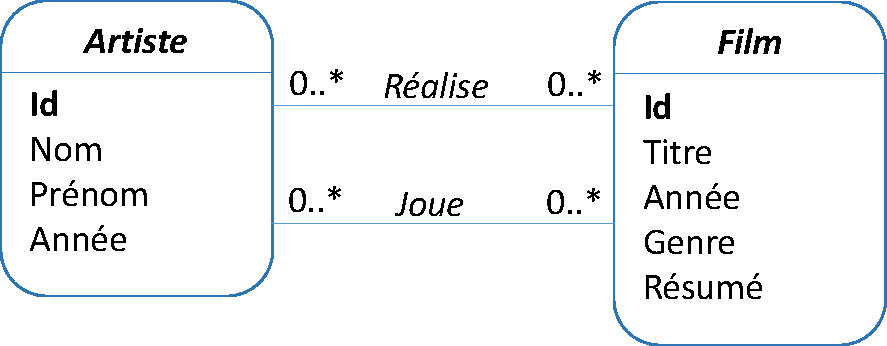
\includegraphics[width=0.7\linewidth]{img/img1}
\end{center}

Les associations sont caractérisées par des cardinalités. La notation \textit{0..*} sur le lien \textit{Réalise}, du côté de l'entité Artiste, signifie qu'un film peut être réalisé par plusieurs artistes, ou aucun. Une notation \textit{0..1} signifierai en revanche qu'un film ne peut être réalisé que par au plus un artiste, \textit{1..1} signifierai un seul artiste.

Les \textbf{clés} sont indiqués en gras, elles permettent d'identifier de manière unique une instance de la table.
\end{frame}

\begin{frame}[fragile]
\frametitle{Tables de jointure}

La mise en place de tables de jointure permet de retrouver les relations entre les instances des tables.

\begin{center}
Table des réalisateurs \\ ~\ \\
\begin{tabular}{|c|c|c|c|}
\hline
\textbf{Id} & \textbf{IdFilm} & \textbf{IdReal1} & \textbf{IdReal2}\\
\hline
1 & 1 & 1 & 2\\
\hline
2 & 2 & 3 & \\
\hline
3 & 3 & 3 &  \\
\hline
4 & 5 & 4 & \\
\hline
5 & 4 & 1 & 2\\
\hline
\end{tabular}
\end{center}

\end{frame}

\begin{frame}[fragile]
\frametitle{Définition d'un schéma relationnel}

Une relation est caractérisée par un \textbf{nom} et se compose d'un ensemble de colonnes désignées par un nom d'\textbf{attribut}. Dans chaque colonne on trouve des valeurs d'un certain \textbf{domaine} (chaînes de caractères, nombres). Enfin on constate que chaque ligne (ou tuple) correspond à une \textbf{entité}.

Ainsi pour le schéma relationnel suivant:\\
Film (titre: string, année: number, genre : string)

\begin{itemize}
 \item \textit{Film} est le \textbf{nom},
 \item \textit{titre}, \textit{année} et \textit{genre} sont des \textbf{attributs},
 \item \textit{sting} et \textit{number} sont des \textbf{domaines}.
 \end{itemize}

('Fargo',1996,'Thriller') est un \textbf{tuple}.

\end{frame}

\section{Le langage SQL}

\begin{frame}[fragile]
\frametitle{Types du langage de données SQL}

\begin{center}
 \begin{tabular}{|c|c|c|}
\hline
Type & Description & Taille \\
\hline
INTEGER & Type des entiers relatifs & 4 octets \\
\hline
SMALLINT & Idem. & 2 octets \\
\hline
BIGINT & Idem. & 8 octets \\
\hline
FLOAT & Flottants simple précision & 4 octets \\
\hline
DOUBLE PRECISION & Flottants double précision & 8 octets \\
\hline
REAL & Synonyme de FLOAT & 4 octets \\
\hline
NUMERIC (M, D) & Numérique avec précision fixe. & M octets \\
\hline
DECIMAL (M, D) & Idem. & M octets \\
\hline
CHAR(M) & Chaînes de longueur fixe & M octets \\
\hline
VARCHAR(M) & Chaînes de longueur variable & $L+1$ avec $L\leq M$ \\
\hline
BIT VARYING & Chaînes d'octets & Longueur de la chaîne \\
\hline
DATE & Date (jour, mois, an) & env. 4 octets \\
\hline
TIME & Horaire (heure, minutes, secondes) & env. 4 octets \\
\hline
DATETIME & Date et heure & 8 octets \\
\hline
YEAR & Année & 2 octets \\
\hline
 \end{tabular}
\end{center}

\end{frame}

\begin{frame}[fragile]
\frametitle{Langage de définition de données SQL}

\textbf{Langage de définition de données SQL}

\begin{GrayBox}[0.85\textwidth]
\begin{semiverbatim}\small
CREATE TABLE eleve (id INT (4) NOT NULL,
                    email VARCHAR (50) NOT NULL,
                    nom VARCHAR (20) NOT NULL,
                    prenom VARCHAR (20),
                    motDePasse VARCHAR (60) NOT NULL,
                    classe VARCHAR (4) DEFAULT 'PTSI',
                    lv1 INT (1) NOT NULL,
                    PRIMARY KEY (Id),
                    FOREIGN KEY (lv1))\end{semiverbatim}\end{GrayBox}

\vspace{-0.5cm}

\textbf{Clés primaire} (\verb? PRIMARY KEY?) \\
Une clé est un attribut qui identifie de manière unique un tuple d'une relation.

\textbf{Clés étrangères} (\verb? FOREIGN KEY?) \\
La norme SQL ANSI permet d'indiquer quelles sont les clés étrangères dans une table, autrement
dit, quels sont les attributs qui font référence à une ligne dans une autre table.
\end{frame}

\begin{frame}[fragile]
\frametitle{Langage de définition de données SQL}

\textbf{Modification d'une table: Ajout d'un champ}

\begin{GrayBox}[0.85\textwidth]
\begin{semiverbatim}\small
ALTER TABLE Internaute ADD region VARCHAR(10)
\end{semiverbatim}
\end{GrayBox}

\textbf{Modification d'une table: Modification d'un champ}

\begin{GrayBox}[0.85\textwidth]
\begin{semiverbatim}\small
ALTER TABLE Internaute MODIFY region VARCHAR(30) NOT NULL
\end{semiverbatim}
\end{GrayBox}

\end{frame}

\begin{frame}[fragile]
\frametitle{Application}

Proposer le code de création d'une table permettant de gérer la lv1. Les attributs seront:
\begin{itemize}
 \item un \textit{id} (clé primaire),
 \item un  \textit{nom},
 \item une \textit{salle}.
\end{itemize}

\begin{GrayBox}[0.85\textwidth]
\begin{semiverbatim}\small
\ifdef{\public}{\uncover<2->{CREATE TABLE lv1 (id INT (1) NOT NULL,
                  nom VARCHAR (30) NOT NULL,
                  salle VARCHAR (30) NOT NULL,
                  PRIMARY KEY (id))}}{\vspace{4cm}}
\end{semiverbatim}
\end{GrayBox}
\end{frame}

\begin{frame}[fragile]
\frametitle{Requêtes SQL}

La suite va prendre pour exemple la base de données des \textit{Villes de France} dont le schéma relationnel est le suivant:\\
Ville (ville\_id:int, ville\_departement:int, ville\_nom\_reel=: char, ville\_code\_postal=int, ville\_population\_2010=int, ville\_longitude\_dms:int , ville\_latitude\_dms:int) (d'autres colonnes sont présentes mais elles ne nous intéressent pas ici).

\begin{itemize}
 \item \verb? FROM ? indique la (ou les) tables dans lesquelles on trouve les attributs utiles à la requête,
 \item \verb? SELECT ? indique la liste des attributs constituant le résultat (* pour tout sélectionner),
 \item \verb? WHERE ? indique les conditions que doivent satisfaire les n-uplets de la base pour faire partie du résultat.
\end{itemize}

\end{frame}

\begin{frame}[fragile]
\frametitle{Requêtes SQL}

Lister les éléments de la base \\

\begin{GrayBox}[0.85\textwidth]
\begin{semiverbatim}\small
SELECT ville_nom_reel, ville_population_2010
FROM villes_france_free
WHERE ville_code_postal=40990
\end{semiverbatim}
\end{GrayBox}

\begin{center}
\begin{tabular}{|c|c|}
\hline
\textbf{ville\_nom\_reel} & \textbf{ville\_population\_2010} \\
\hline
Saint-Vincent-de-Paul & 2997 \\
\hline
Téthieu & 656 \\
\hline
Gourbera & 356 \\
\hline
Herm & 1044 \\
\hline
Mées & 1736 \\
\hline
Saint-Paul-lès-Dax & 12409 \\
\hline
Angoumé & 288 \\
\hline
\end{tabular}
\end{center}

\end{frame}

\begin{frame}[fragile]
\frametitle{Requêtes SQL}

Modifier l'affichage des attributs.

\begin{GrayBox}[0.85\textwidth]
\begin{semiverbatim}\small
SELECT ville_nom_reel as 'Ville',
ville_population_2010/1000 AS 'Population en milliers'
FROM villes_france_free
WHERE ville_code_postal=40990 and ville_population_2010>1000
\end{semiverbatim}
\end{GrayBox}

\begin{center}
\begin{tabular}{|c|c|}
\hline
\textbf{Ville} & \textbf{Population en milliers} \\
\hline
Herm & 1.0440 \\
\hline
Mées & 1.7360 \\
\hline
Saint-Vincent-de-Paul & 2.9970 \\
\hline
Saint-Paul-lès-Dax & 12.4090 \\
\hline
\end{tabular}
\end{center}

\end{frame}

\begin{frame}[fragile]
\frametitle{Requêtes SQL}

Recherche dans une table.

\begin{GrayBox}[0.85\textwidth]
\begin{semiverbatim}\small
SELECT ville_nom_reel as 'Ville',ville_code_postal as 'Code Postal'
FROM `villes_france_free`
WHERE `ville_nom_reel`='Saint-Vincent-de-Paul'
\end{semiverbatim}
\end{GrayBox}

\begin{center}
\begin{tabular}{|c|c|}
\hline
\textbf{Ville} & \textbf{Code Postal} \\
\hline
Saint-Vincent-de-Paul & 33440 \\
\hline
Saint-Vincent-de-Paul & 40990 \\
\hline
\end{tabular}
\end{center}

Éviter les doublons.

\begin{minipage}{0.7\linewidth}
\begin{GrayBox}[0.85\textwidth]
\begin{semiverbatim}\small
SELECT DISTINCT ville_nom_reel as 'Ville'
FROM `villes_france_free`
WHERE `ville_nom_reel`='Saint-Vincent-de-Paul'
\end{semiverbatim}
\end{GrayBox}
\end{minipage}\hfill
\begin{minipage}{0.25\linewidth}
\begin{center}
\begin{tabular}{|c|c|}
\hline
\textbf{Ville} \\
\hline
Saint-Vincent-de-Paul \\
\hline
\end{tabular}
\end{center}
\end{minipage}
\end{frame}

\begin{frame}[fragile]
\frametitle{Requêtes SQL}

Affichage trié:

\begin{GrayBox}[0.85\textwidth]
\begin{semiverbatim}\small
SELECT ville_nom_reel, ville_population_2010
FROM villes_france_free
WHERE ville_code_postal=40990 ORDER BY ville_population_2010
\end{semiverbatim}
\end{GrayBox}

\begin{center}
\begin{tabular}{|c|c|}
\hline
\textbf{ville\_nom\_reel} & \textbf{ville\_population\_2010} \\
\hline
Angoumé & 288 \\
\hline
Gourbera & 356 \\
\hline
Téthieu & 656 \\
\hline
Herm & 1044 \\
\hline
Mées & 1736 \\
\hline
Saint-Vincent-de-Paul & 2997 \\
\hline
Saint-Paul-lès-Dax & 12409 \\
\hline
\end{tabular}
\end{center}

Le tri dans l'ordre descendant s'effectue en ajoutant DESC, à la suite des paramètres de classement.

\end{frame}

\begin{frame}[fragile]
\frametitle{Requêtes SQL}

Calcul de somme:

\begin{GrayBox}[0.85\textwidth]
\begin{semiverbatim}\small
SELECT SUM(ville_population_2010) AS 'Population Totale 40990'
FROM villes_france_free
WHERE ville_code_postal=40990
\end{semiverbatim}
\end{GrayBox}

\begin{center}
\begin{tabular}{|c|}
\hline
\textbf{Population Totale 40990} \\
\hline
19486 \\
\hline
\end{tabular}
\end{center}

Calcul de moyenne:

\begin{GrayBox}[0.85\textwidth]
\begin{semiverbatim}\small
SELECT AVG(ville_population_2010) AS 'Population Moyenne 40990'
FROM villes_france_free
WHERE ville_code_postal=40990
\end{semiverbatim}
\end{GrayBox}

\begin{center}
\begin{tabular}{|c|}
\hline
\textbf{Population Moyenne 40990} \\
\hline
2783.7143 \\
\hline
\end{tabular}
\end{center}

\end{frame}

\begin{frame}[fragile]
\frametitle{Requêtes SQL}

Compter les valeurs:

\begin{GrayBox}[0.85\textwidth]
\begin{semiverbatim}\small
SELECT COUNT(ville_nom_reel) AS 'Nombre de villes'
FROM villes_france_free
WHERE ville_code_postal=40990
\end{semiverbatim}
\end{GrayBox}

\begin{center}
\begin{tabular}{|c|}
\hline
\textbf{Nombre de villes} \\
\hline
7 \\
\hline
\end{tabular}
\end{center}

\begin{minipage}{0.65\linewidth}
\begin{GrayBox}[0.9\textwidth]
\begin{semiverbatim}\small
SELECT ville_departement AS 'Département',
COUNT(ville_id) as 'Nb villes'
FROM villes_france_free
WHERE ville_departement > 40
    AND ville_departement < 45
GROUP BY ville_departement
\end{semiverbatim}
\end{GrayBox}
\end{minipage}\hfill
\begin{minipage}{0.3\linewidth}

\begin{center}
\begin{tabular}{|c|c|}
\hline
\textbf{Département} & \textbf{Nb villes} \\
\hline
41 & 291 \\
\hline
42 & 327 \\
\hline
43 & 260 \\
\hline
44 & 221 \\
\hline
\end{tabular}
\end{center}
\end{minipage}

\end{frame}

\begin{frame}[fragile]
\frametitle{Requêtes SQL}

Limiter le nombre de réponse

\begin{minipage}{0.7\linewidth}
\begin{GrayBox}[0.85\textwidth]
\begin{semiverbatim}\small
SELECT ville_nom_reel AS Ville,
    ville_population_2010 AS Population
FROM villes_france_free
ORDER BY ville_population_2010 DESC LIMIT 1
\end{semiverbatim}
\end{GrayBox}
\end{minipage}\hfill
\begin{minipage}{0.25\linewidth}
\begin{center}
\begin{tabular}{|c|c|}
\hline
\textbf{Ville} & \textbf{Population} \\
\hline
Paris & 2243833 \\
\hline
\end{tabular}
\end{center}
\end{minipage}

Rechercher le maximum d'une liste

\begin{minipage}{0.7\linewidth}
\begin{GrayBox}[0.9\textwidth]
\begin{semiverbatim}\small
SELECT ville_nom_reel AS Ville,
    ville_population_2010 AS Population
FROM villes_france_free
WHERE ville_population_2010=
    (SELECT max(ville_population_2010)
        FROM villes_france_free)
\end{semiverbatim}
\end{GrayBox}
\end{minipage}\hfill
\begin{minipage}{0.25\linewidth}
\begin{center}
\begin{tabular}{|c|c|}
\hline
\textbf{Ville} & \textbf{Population} \\
\hline
Paris & 2243833 \\
\hline
\end{tabular}
\end{center}
\end{minipage}
\end{frame}

\begin{frame}[fragile]
\frametitle{Requêtes SQL}

Recherche de plusieurs maximums.

\begin{GrayBox}[0.85\textwidth]
\begin{semiverbatim}\small
SELECT ville_departement AS Département, ville_nom_reel AS Ville,
    ville_population_2010 AS Population
FROM villes_france_free v,
    (SELECT max(ville_population_2010) AS Max FROM villes_france_free
        WHERE ville_departement >=40 AND ville_departement <45
            GROUP BY ville_departement) m
WHERE v.ville_population_2010=m.Max
\end{semiverbatim}
\end{GrayBox}

\begin{center}
\begin{tabular}{|c|c|c|}
\hline
\textbf{Département} & \textbf{Ville} & \textbf{Population} \\
\hline
40 & Mont-de-Marsan & 31225 \\
\hline
41 & Blois & 46492 \\
\hline
42 & Saint-Étienne & 171260 \\
\hline
43 & Le Puy-en-Velay & 18521 \\
\hline
44 & Nantes & 284970 \\
\hline
\end{tabular}
\end{center}

\end{frame}

\begin{frame}[fragile]
\frametitle{Requêtes SQL}

Utilisation de \verb? HAVING ? pour limiter les résultats avec des \verb? SUM ?, \verb? AVG ?,...

\begin{GrayBox}[0.85\textwidth]
\begin{semiverbatim}\small
SELECT ville_departement AS Département,
    SUM(ville_population_2010) AS Population
FROM villes_france_free
GROUP BY ville_departement
HAVING SUM(ville_population_2010)<100000
\end{semiverbatim}
\end{GrayBox}

\begin{center}
\begin{tabular}{|c|c|}
\hline
\textbf{Département} & \textbf{Population} \\
\hline
48 & 77082 \\
\hline
975 & 6080 \\
\hline
\end{tabular}
\end{center}

\end{frame}

\section{Jointure et requêtes multiples}

\begin{frame}[fragile]
\frametitle{Requêtes SQL}

Des tables sont ajoutées afin de gérer les régions et les départements.

\begin{GrayBox}[0.85\textwidth]
\begin{semiverbatim}\small
SELECT departement_nom as Département, departement_code as Numéro
FROM `departement`
WHERE departement_code < 50 AND departement_code >= 40
\end{semiverbatim}
\end{GrayBox}

\begin{center}
\begin{tabular}{|c|c|}
\hline
\textbf{Département} & \textbf{Numéro} \\
\hline
Landes & 40 \\
\hline
Loir-et-Cher & 41 \\
\hline
Loire & 42 \\
\hline
Haute-Loire & 43 \\
\hline
Loire-Atlantique & 44 \\
\hline
Loiret & 45 \\
\hline
Lot & 46 \\
\hline
Lot-et-Garonne & 47 \\
\hline
Lozère & 48 \\
\hline
Maine-et-Loire & 49 \\
\hline
\end{tabular}
\end{center}

\end{frame}

\begin{frame}[fragile]
\frametitle{Requêtes SQL}
\begin{GrayBox}[0.85\textwidth]
\begin{semiverbatim}\small
SELECT `Id_region`,`NCCENR` AS Nom
FROM `regions`
WHERE `Id_region`>40
\end{semiverbatim}
\end{GrayBox}

\begin{center}
\begin{tabular}{|c|c|}
\hline
Id\_region & Nom \\
\hline
44 & Alsace-Champagne-Ardenne-Lorraine \\
\hline
52 & Pays de la Loire \\
\hline
53 & Bretagne \\
\hline
75 & Aquitaine-Limousin-Poitou-Charentes \\
\hline
76 & Languedoc-Roussillon-Midi-Pyrénées \\
\hline
84 & Auvergne-Rhône-Alpes \\
\hline
93 & Provence-Alpes-Côte d'Azur \\
\hline
94 & Corse \\
\hline
\end{tabular}
\end{center}
\end{frame}

\begin{frame}[fragile]
\frametitle{Requêtes SQL}


\begin{GrayBox}[0.85\textwidth]
\begin{semiverbatim}\small
SELECT * FROM `jointure departement-region` WHERE id_region=75
\end{semiverbatim}
\end{GrayBox}

\begin{center}
\begin{tabular}{|c|c|}
\hline
\textbf{id\_departement} & \textbf{id\_region} \\
\hline
16 & 75 \\
\hline
17 & 75 \\
\hline
19 & 75 \\
\hline
23 & 75 \\
\hline
24 & 75 \\
\hline
33 & 75 \\
\hline
40 & 75 \\
\hline
47 & 75 \\
\hline
64 & 75 \\
\hline
79 & 75 \\
\hline
86 & 75 \\
\hline
87 & 75 \\
\hline
\end{tabular}
\end{center}
\end{frame}

\begin{frame}[fragile]
\frametitle{Requêtes SQL}

Des tables sont ajoutées afin de gérer les régions et les départements.

\begin{GrayBox}[0.85\textwidth]
\begin{semiverbatim}\small
SELECT v.ville_nom_reel, d.departement_nom, v.ville_population_2010
FROM villes_france_free v
JOIN departement d ON d.departement_code=v.ville_departement
WHERE v.ville_population_2010>400000
ORDER BY v.ville_population_2010 DESC
\end{semiverbatim}
\end{GrayBox}

\begin{center}
\begin{tabular}{|c|c|c|}
\hline
\textbf{ville\_nom\_reel} & \textbf{departement\_nom} & \textbf{ville\_population\_2010} \\
\hline
Paris & Paris & 2243833 \\
\hline
Marseille & Bouches-du-Rhône & 850726 \\
\hline
Lyon & Rhône & 484344 \\
\hline
Toulouse & Haute-Garonne & 441802 \\
\hline
\end{tabular}
\end{center}
\end{frame}

\begin{frame}[fragile]
\frametitle{Requêtes SQL}
\begin{GrayBox}[0.85\textwidth]
\begin{semiverbatim}\small
SELECT v.ville_nom_reel AS Ville, d.departement_nom AS Département,
r.NCCENR AS Région, v.ville_population_2010 AS Population
FROM villes_france_free v
JOIN departement d JOIN regions r JOIN jointure_departement_region j
    ON d.departement_code=v.ville_departement
    AND d.departement_code=j.id_departement
    AND r.Id_region=j.id_region
WHERE v.ville_population_2010>400000
ORDER BY v.ville_population_2010 DESC
\end{semiverbatim}
\end{GrayBox}

\begin{center}
\begin{tabular}{|c|c|c|c|}
\hline
\textbf{Ville} & \textbf{Département} & \textbf{Région} & \textbf{Population} \\
\hline
Paris & Paris & Ile de France & 2243833 \\
\hline
Marseille & Bouches-du-Rhône & Provence-Alpes-Côte d'Azur & 850726 \\
\hline
Lyon & Rhône & Auvergne-Rhône-Alpes & 484344 \\
\hline
Toulouse & Haute-Garonne & Languedoc-Roussillon-Midi-Pyrénées & 441802 \\
\hline
\end{tabular}
\end{center}

\end{frame}

\section{Insérer, modifier, supprimer}

\begin{frame}[fragile]
\frametitle{Requêtes SQL}

Modification d'une table (gestion de la LV1).

Insérer une ligne.

\begin{GrayBox}[0.85\textwidth]
\begin{semiverbatim}\small
INSERT INTO lv1 VALUES (1, 'Anglais', 'B302')
\end{semiverbatim}
\end{GrayBox}

Modifier une ligne.

\begin{GrayBox}[0.85\textwidth]
\begin{semiverbatim}\small
UPDATE lv1 SET salle='B306' WHERE Id=1
\end{semiverbatim}
\end{GrayBox}

Supprimer une ligne.

\begin{GrayBox}[0.85\textwidth]
\begin{semiverbatim}\small
DELETE FROM lv1 WHERE Id=1
\end{semiverbatim}
\end{GrayBox}     
\end{frame}

\end{document}

